\section{Sha256}
Este algoritmo es utilizado principalmente en el área de seguridad de la información. Desde el punto de vista del usuario el algoritmo recibe una tira de bytes como input (conocida como message o mensaje) y devuelve una tira de 256 bits usualmente expresado en bloques de hexadecimal (conocido como message digest). Por ejemplo: \\

\begin{tabular}{|c | c |}
\hline
 Mensaje  & Message Digest \\
\hline
"This is a test." & 0xc7be1ed902fb8dd4d48997c6452f5d7e509fbcdbe2808b16bcf4edce4c07d14e\\
\hline
"This is a test" & 0x71d2097303bd0714f6eee360f283643d3d1c6418fb626406347c671b21053a90 \\
\hline
"This is a est" & 0xd8e64876b6151251624a4a6d65ad558220c74c6638c73172d3126b655149519a \\
\hline
\end{tabular} \\
\textit{Como se puede ver en el ejemplo, un pequeño cambio en el input genera grandes cambios en el output.}\\

Sha256 forma parte de la familia de funciones conocidas como \textit{funciones de hash o one way functions}. Estas cumplen con un conjunto de propiedades importantes \cite{CrypEng} desde el punto de vista de la seguridad. Suponiendo que $M$ es el mensaje, $h$ es el resultado de aplicar la función a $M$ y $H$ es la función de hash:
\begin{itemize}
    \item Dado $M$, es computacionalmente sencillo obtener $h$.
    \item Dado $h$, es computacionalmente difícil obtener $M$ tal que $H(M)= h$.
    \item Dado $M$, es computacionalmente difícil obtener otro mensage, $M'$, tal que $H(M) = H(M')$.
    \item Es improbable encontrar de forma aleatoria dos mensajes distintos, $M$ y $M'$, tal que $H(M) = H(M')$.
\end{itemize}

Estas propiedades se pueden aprovechar para detectar cambios en tiras de bytes con solo conocer los 256 bits devueltos al aplicar la función de hash a los datos enviados ($H(M)$); entonces el receptor puede estar muy seguro que los datos recibidos no fueron alterados por algún tercero o algún error en el canal de transmisión, etc. Un ejemplo de uso importante se da cuando se quiere enviar un archivo desde un servidor hasta un cliente, el cual quiere verificar si los datos recibidos son correctos. Estos datos podrían ser desde una página web hasta una pieza crítica de software. Más foralmente, $A$ quiere mandar a $B$ el mensaje $M$; $B$ quiere estar seguro de que el mensaje recibido $M'$ cumple $M = M'$. La solución es que $A$ comunique $H(M)$ mediante un canal seguro a $B$ y luego éste calcula $H(M')$, luego, si $H(M) = H(M')$ se puede afirmar con un alto grado de seguridad que $M = M'$. Estamos suponiendo que la longitud de $H(M)$ es menor que $M$, lo que es usualmente cierto en la práctica (de otra manera se podría haber usado el canal seguro para mandar el mensaje completo). Un ejemplo importante en la práctica es la publicación en alguna página web del hash de un paquete de actualización, que una vez descargado puede aplicarsele el hash y asegurarse que no haya sido modificado. Muchas veces este procedimiento se realiza automáticamente.  \\
\indent Otro uso importante es el almacenamiento de passwords. Si tenemos un método de autenticación que usa passwords, no es recomendable guardarlos como texto plano, ya que esto disminuye considerablemente la seguridad del sistema (especialmente si el mismo es compartido por varios usuarios). Una solución es guardar el resultado de aplicar una función hash al password y luego para saber si una string coincide con el password, se comparan los resultados de los hash en vez de comparar el texto plano. Más formalmente, si el password es $P$, se guarda $H(P)$; luego una string $P'$ será CONSIDERADO el password correcto si y solo sí $H(P) = H(P')$.\\
\indent Claramente los sistemas no son completamente seguros, ya que podrían encontrarse colisiones y romper así la seguridad del sistema (es decir encontrar un mensaje $M'$ tal que $H(M') = H(M)$ pero $M \neq M'$), pero esto, por las propiedades enumeradas anteriormente es extramadamente improbable, e intentar encontrar dicha colisión mediante un algoritmo es intractable y muy costoso en la práctica. \\

Algunas aplicaciones y sistemas populares que usan la función hash sha256 son la autenticación de paquetes de software en Debian Gnu/Linux y el protocolo de la moneda virtual Bitcoin (el uso en este caso es distinto de los explicados anteriormente).  \\

\subsection{Pseudocódigo}
\label{sec:shapseudo}

En esta sección explicamos con más detalle el algoritmo y presentamos un pseudocódigo del mismo \cite{Fips}.\\

Como se mencionó anteriormente, sha256 recibe como input una tira de bits y devuelve una tira de $256$ bits usualmente expresados en bloques de hexagesimal. El input o mensaje, es partido en bloques de $512$ bits cada uno. En caso de que la longitud del mensaje no sea múltiplo de $512$ bits, se le aplica padding al mensaje original, lo que consta de agregar el bit $1$ al final del mensaje seguido de $k$ bits en cero, donde $k$ es la mínima solución a la ecuación $l + 1 + k \equiv 896$ mod $1024$ y luego la expresión en binario de $l$ en $128$ bits, con $l$ la longitud del mensaje original en bits. Por ejemplo, si el mensaje es ''abc'' codificado en ASCII, entonces $l = 24$, por lo que al mensaje se le deben agregar un bit en $1$, $871$ bits en cero y luego, en $128$ bits, la longitud del mensaje en binario.\\ De ahora en más podemos suponer que $l$ es múltiplo de $512$. \\
\indent Luego del preproceso (aplicación del padding si es necesario), se cargan los valores de hash iniciales en una variable $H$,            
                                    $$ H^{(0)}_0 = \texttt{0x6a09e667} $$
                                    $$ H^{(1)}_0 = \texttt{0xbb67ae85} $$
                                    $$ H^{(2)}_0 = \texttt{0x3c6ef372} $$
                                    $$ H^{(3)}_0 = \texttt{0xa54ff53a} $$
                                    $$ H^{(4)}_0 = \texttt{0x510e527f} $$
                                    $$ H^{(5)}_0 = \texttt{0x9b05688c} $$
                                    $$ H^{(6)}_0 = \texttt{0x1f83d9ab} $$
                                    $$ H^{(7)}_0 = \texttt{0x5be0cd19} $$

y para cada bloque del mensaje se aplica el procedimiento que llamaremos de ahora en más $\texttt{process\_bock}$, que actualiza los valores de $H^{(i)}$ en cada pasada, obteniendo el resultado final luego del último bloque. Antes de analizar en más detalle el método \texttt{process\_bock}, se dan algunas definiciones necesarias sobre funciones y variables a utilizar en el pseudocódigo. Se usan las siguientes funciones sobre parámetros de $32$ bits, devolviendo también valores de $32$ bits,
$$Ch ( x , y , z ) = (x \land y) \oplus (\neg x \land z)$$
$$Maj ( x , y , z ) = (x \land y) \oplus (x \land z) \oplus (y \land z) $$
$$ROTR^n(x) = (x >> n) \lor (x << 32 - n) $$
$$\sum^{\{256\}}_0(x) = ROTR^2(x) \oplus  ROTR^{13}(x) \oplus  ROTR^{22}(x)$$
$$\sum^{\{256\}}_1(x) = ROTR^6(x) \oplus  ROTR^{11}(x) \oplus  ROTR^{25}(x)$$
$$\sigma^{\{ 256\}}_0(x) = ROTR^7(x) \oplus  ROTR^{18}(x) \oplus  x >> 3 $$
$$\sigma^{\{ 256\}}_1(x) = ROTR^{17}(x) \oplus  ROTR^{19}(x) \oplus  x >> 10$$


Las variables a usar son $\; \; \; a, b, \dots , h \; \text{variables temporales de $32$ bits}$
$$H^{(i)} \; \text{el valor hash actual, en la $i$-ésima iteración} $$
$$H^{(i)}_j \; \text{la $j$-ésima palabra de $32$-bits del valor hash en la $i$-ésima iteración} $$
$$M^i_j \; \text{la $j$-ésima palabra de $32$-bits del $i$-ésimo bloque del mensaje} $$
$$W_t \; \text{la $t$-ésima palabra de $32$ bits del message schedule} $$
$$K_t \; \text{la $t$-ésima palabra de $32$ bits de una constante definida en el standard \cite{Fips}} $$

Con todo lo anterior puede presentarse el pseudocódigo del procedimiento \texttt{process\_block}: 
\begin{algorithm}[H]
\caption{process\_block}
\begin{algorithmic}[0]
    \State 1)- Preparar el message schedule ($W_t$)
    \State
    \State \indent $W_t = \left\{ \begin{array}{lcc}
                            M^{(i)}_t &   si  & 0 \leq t \leq 15 \\
                         \\ \sigma_1^{\{256\}}(W_{t-2}) + W_{t-7} + \sigma_0^{\{256\}}(W_{t-15}) + W_{t-16} &  si & 16 \leq t \leq 63 \\
                     \end{array} \right. $                   
    \State 2)- Inicializar las 8 variables temporales con el hash actual (almacenado en $H^{(i-1)}$)
    \State \indent $a = H^{(i-1)}_0 $
    \State \indent $b = H^{(i-1)}_1 $
    \State \indent $c = H^{(i-1)}_2 $
    \State \indent $d = H^{(i-1)}_3 $
    \State \indent $e = H^{(i-1)}_4 $
    \State \indent $f = H^{(i-1)}_5 $
    \State \indent $g = H^{(i-1)}_6 $
    \State \indent $h = H^{(i-1)}_7 $
    \State 3)-
    \For{$t=0$ to $63$}
        \State $T_1 = h + \sum^{\{256\}}_1(e) + Ch(e, f, g) + K^{\{256\}}_t + W_t $
        \State $T_2 = \sum^{\{256\}}_0(a) + Maj(a,b,c)$
        \State $h = g$
        \State $g = f$
        \State $f = e$
        \State $e = d + T_1$
        \State $d = c$
        \State $c = b$
        \State $b = a$
        \State $a = T 1 + T_2$
    \EndFor
    \State
    \State 4)- Actualizar el i-ésimo valor hash
    \State  \indent $H^{(i)}_0  = a + H^{(i-1)}_0 $
    \State  \indent $H^{(i)}_1  = b + H^{(i-1)}_1 $
    \State  \indent $H^{(i)}_2  = c + H^{(i-1)}_2 $
    \State  \indent $H^{(i)}_3  = d + H^{(i-1)}_3 $
    \State  \indent $H^{(i)}_4  = e + H^{(i-1)}_4 $
    \State  \indent $H^{(i)}_5  = f + H^{(i-1)}_5 $
    \State  \indent $H^{(i)}_6  = g + H^{(i-1)}_6 $
    \State  \indent $H^{(i)}_7  = h + H^{(i-1)}_7 $
\end{algorithmic}
\end{algorithm}

El resultado final es, suponiendo que hay $N$ bloques, la concatenación de $H$, es decir,
            $$ H^{(N)}_0 \left\| H^{(N)}_1 \right\| H^{(N)}_2 \left\| H^{(N)}_3 \right\| H^{(N)}_4 \left\| H^{(N)}_5 \right\| H^{(N)}_6 \left\| H^{(N)}_7 \right. $$

\subsection{Implementaciones}
Se realizaron cuatro implementaciones de \texttt{process\_block}, todas compartiendo el código que realiza padding e inicialización de la variable $H$, una en lenguage C y en las otras ensamblador de IA64. Las implementaciones se nombraron \texttt{process\_block} (lenguage C), \texttt{process\_block\_asm}, \texttt{process\_block\_asm\_simd} en la cual se usaron técnicas SIMD y \texttt{process\_block\_simd\_stich} en la cual se uso además una técnica llamada function stitching . En todos los casos la función recibe 2 parámetros, un puntero al bloque del mensaje y la variable que mantiene el estado actual del hash ($H$), que se implementa como un array de ocho \texttt{unsigned int}.\\

\subsubsection{Implementación en C}
\label{sec:impshac}
En este caso, el código sigue el formato del standard que define Sha256 \cite{Fips}. Se usaron \texttt{unsigned int} para las palabras de $32$ bits del standard y punteros a \texttt{unsigned char} para el mensaje. La única dificultad que tuvo que ser superada, que también está presente en las otras implementaciones, es el uso de big endian en la definición del standard, lo que contrasta con la arquitectura usada, que es little endian. Por esta razón deben invertirse el orden de los datos al traerlos desde las porciones memoria que contienen el mensaje durante el message schedule. Para hacerlo se usa el siguiente código, en donde $W$ y $M$ tienen los significados dados en la sección \ref{sec:shapseudo}, pero con tipos de C \texttt{unsigned int$^*$} y \texttt{unsigned char$^*$} respectivamente, 
\begin{verbatim} 
        for (t = 0; t < 16; t++) // problemas con endianness                                                 
            W[t] = (M[4*t] << 24) | (M[4*t + 1] << 16) | (M[4*t + 2] << 8) | M[4*t + 3];
\end{verbatim}
\indent Es importante destacar que el procedimiento $\texttt{process\_block\_C}$ se compila usando el flag $\texttt{-O3}$ que genera en este caso, código máquina que usa instrucciones y demás recursos de las extenciones SIMD del procesador.


\subsubsection{Implementación en ensamblador (no SIMD)}
El código sigue el formato del standard \cite{Fips}, consta de 4 partes como en la sección \ref{sec:shapseudo}, las cuales se pueden diferenciar en el mismo. \\
\indent En la sección 1), correspondiente al cálculo del message schedule, una vez que los datos están en registros internos del procesador, el cómputo que corresponde a la función auxiliar $\sigma$ es hecha en los mismos, aunque es necesario traer datos de la memoria correspondientes a la variable $W$. \\
\indent Para las secciónes 2), 3) y 4) del pseudocódigo, se representaron las variables temporales $a, \dots, h$ en las doublewords bajas de los registros de propósito general siendo $$\texttt{a} = \texttt{eax}, \texttt{b} = \texttt{edx}, \texttt{c} = \texttt{esi}, \texttt{d} = \texttt{edi}, \texttt{e} = \texttt{r8d}, \texttt{f} = \texttt{r9d}, \texttt{g} = \texttt{r10d}, \texttt{h} = \texttt{r11d}  $$ usando algunos de los restantes para mantener temporalmente el resultado de algunas operaciones. De esta manera, para calcular, por ejemplo, $\sum^{\{256\}}_1(e)$ se computa 
\begin{verbatim}
                 mov r14d, r8d
                 mov r15d, r8d
                 ror r14d, 6
                 ror r15d, 11
                 xor r14d, r15d
                 mov r15d, r8d
                 ror r15d, 25
                 xor r14d, r15d
\end{verbatim}

quedando el resutado en \texttt{r14d}. Al computar las distintas funciones auxiliares, se intentó ordenar las operaciones de manera que las dependencias de datos entre las mismas sean las menores posibles, la cantidad de registros usados para mantener las variables $ \texttt{a}, \dots, \texttt{h} $ y los usados para mantener resultados intermedios, hace que no se puedan usar registros adicionales para romper estas dependencias.

\subsubsection{Implementación en ensamblador usando SIMD}
\label{sec:shaimpSIMD}
Esta implementación utiliza las extenciones SIMD de intel (sse, sse2, ssse3) para optimizar ciertas secciones críticas del código. La principal aplicación de esta técnica está en el cómputo del message schedule, que en la versión de C se hace del siguiente modo
\begin{verbatim} 
        for (t = 0; t < 16; t++) // problemas con endianness                                                 
            W[t] = (M[4*t] << 24) | (M[4*t + 1] << 16) | (M[4*t + 2] << 8) | M[4*t + 3];
\end{verbatim}
\begin{verbatim} 
        for (t = 16; t < 64; t++)
            W[t] = sig1(W[t-2]) + W[t-7] + sig0(W[t-15]) + W[t-16];
\end{verbatim}

Para optimizar el primer ciclo, es importante disminuir la cantidad de accesos a memoria, para eso, teniendo en cuenta que se leen $64$ bytes en posiciones adyacentes de memoria, se lo hace de la siguiente manera, aprovechando los registros $\texttt{xmm}$ de $16$ bytes cada uno
\begin{verbatim}
        movdqa xmm0, [rdi]
        movdqa xmm1, [rdi+16]
        pshufb xmm0, xmm13
        movdqa xmm2, [rdi+32]
        pshufb xmm1, xmm13
        movdqa xmm3, [rdi+48]
        pshufb xmm2, xmm13
        pshufb xmm3, xmm13
\end{verbatim}
donde xmm13 contiene la máscara
\begin{verbatim}
 db 0x3, 0x2, 0x1, 0x0, 0x7, 0x6, 0x5, 0x4, 0xb, 0xa, 0x9, 0x8, 0xf, 0xe, 0xd, 0xc
\end{verbatim}
y el registro $\texttt{rdi}$ apunta al mensaje. Como se puede ver, se usa la instrucción $\texttt{pshufb}$ para reacomodar los bytes a big endian. Es importante recordar que $\texttt{W[t]}$ es de $4$ bytes.\\
\indent El segundo ciclo consta de $48$ iteraciones, en las cuales se trata con operaciones sobre $32$ bits, que pueden implementarse en SIMD sin mucha dificultad.\\
\indent Debido a que para calcular $\texttt{W[t]}$ se requiere de $\texttt{W[t-2]}$, sólo se puede calcular en paralelo $\texttt{W[t]}$ y $\texttt{W[t+1]}$, por lo que es necesario computarlos aparte para poder obtener $\texttt{W[t+2]}$ y $\texttt{W[t+3]}$, en particular es necesario obtener $\sigma_1(\texttt{W[t-1]})$ y $\sigma_1(\texttt{W[t-2]})$ para poder calcular $\texttt{W[t+2]}$ y $\texttt{W[t+3]}$. Las demás operaciones pueden hacerse en paralelo, $4$ al mismo tiempo. \\
\indent La ejecución de $4$ iteraciones de este ciclo se encapsularon en la macro $\texttt{iteracion\_segundo\_ciclo}$. Este recibe como parámetros $4$ registros $\texttt{xmm}$ que guardan los $\texttt{W's}$ computados anteriormente que son necesarios. El resultado se guarda en el primer parámetro ($\%1$ en la syntaxis de NASM) y es $\texttt{W[t]} \dots \texttt{W[t+3]}$.\\
\indent Para mayor claridad, una representación gráfica del código, asumiendo que los parámetros son 
$\texttt{xmm0}$, $\texttt{xmm1}$, $\texttt{xmm2}$, $\texttt{xmm3}$, con los siguientes datos
$$\texttt{xmm0} = \texttt{W[t-13]} | \texttt{W[t-14]} | \texttt{W[t-15]} | \texttt{W[t-16]}$$
$$\texttt{xmm1} = \texttt{W[t-9]} | \texttt{W[t-10]} | \texttt{W[t-11]} | \texttt{W[t-12]}$$
$$\texttt{xmm2} = \texttt{W[t-5]} | \texttt{W[t-6]} | \texttt{W[t-7]} | \texttt{W[t-8]}$$
$$\texttt{xmm3} = \texttt{W[t-1]} | \texttt{W[t-2]} | \texttt{W[t-3]} | \texttt{W[t-4]}$$

\noindent donde cada separación indica un doubleword distinto y $\texttt{t}$ es el mayor que cumple que $\texttt{W[t]}$ fue calculado. Cabe destacar que esta macro se usa luego de haber calculado $\texttt{W[0]} \dots \texttt{W[15]}$ en el primer ciclo. 

\begin{algorithm}[H]
\caption{iteración\_segundo\_ciclo}
\begin{algorithmic}[0]
    \State -Copio xmm3 a xmm4-
    \State $ \texttt{xmm4} = \texttt{W[t-1]} | \texttt{W[t-2]} | \texttt{W[t-3]}  |\texttt{W[t-4]} $
    \State
    \State -Acomodo los datos necesarios en xmm4 usando $palignr  \; \; xmm4, xmm2, 4$ (ver \cite{manualIntelinst} \cite{shaintelimp})- 
    \State $\texttt{xmm4} = \texttt{W[t-4]} | \texttt{W[t-5]} | \texttt{W[t-6]} | \texttt{W[t-7]} $
    \State
    \State -Sumo xmm0 y xmm4, lo guardo en xmm4-
    \State $\texttt{xmm4} = \texttt{W[t-4] + W[t-13]}|\texttt{W[t-5] + W[t-14]}|\texttt{W[t-6] + W[t-15]}|\texttt{W[t-7] + W[t-16]} $
    \State
    \State -Muevo xmm3 a xmm5-
    \State $ \texttt{xmm5} = \texttt{W[t-1]} | \texttt{W[t-2]} | \texttt{W[t-3]}  |\texttt{W[t-4]} $
    \State 
    \State -Acomodo los datos necesarios en xmm5 usando $palignr \; \; xmm5, xmm0, 4$- 
    \State $ \texttt{xmm5} = \texttt{W[t-12]} | \texttt{W[t-13]} | \texttt{W[t-14]}  |\texttt{W[t-15]} $
    \State
    \State -Calculo $\sigma_0(\texttt{W[t-15]})$, $\sigma_0(\texttt{W[t-15]})$, $\sigma_0(\texttt{W[t-15]})$, $\sigma_0(\texttt{W[t-15]})$ en paralelo -
    \State $ \texttt{xmm5} = \sigma_0(\texttt{W[t-12]}) | \sigma_0(\texttt{W[t-13]}) | \sigma_0(\texttt{W[t-14]}) |\sigma_0(\texttt{W[t-15]}) $
    \State
    \State -Sumo $\texttt{xmm5}$ y $\texttt{xmm4}$, solo falta calcular y sumar las $\sigma_1$-
    \State $ \texttt{xmm5} = \texttt{ W[t-4] + W[t-13] + } \sigma_0(\texttt{W[t-12]}) |\texttt{W[t-5] + W[t-14] + } \sigma_0(\texttt{W[t-13]})| $
    \State \indent \indent $ \texttt{W[t-6] + W[t-15] +} \sigma_0(\texttt{W[t-14]})|\texttt{W[t-7] + W[t-16] +} \sigma_0(\texttt{W[t-14]})$
    \State
    \State -Calculo las $\sigma_1$, como se explicó anteriorente solo se pueden calcular 2 en paralelo-
    \State -Calculo primero $\sigma_1(\texttt{W[t-2]})$ y $\sigma_1(\texttt{W[t-1]})$, necesito $\texttt{W[t-1]}$ y $\texttt{W[t-2]}$ -
    \State $ \texttt{xmm0} = \texttt{xmm3} = \texttt{W[t-1]} | \texttt{W[t-2]} | \texttt{W[t-3]}  |\texttt{W[t-4]} $
    \State -Usando shifts obtengo lo que necesito-
    \State $\texttt{xmm0} = 0 | 0 | \texttt{W[t-1]}  |\texttt{W[t-2]} $
    \State -Aplico $\sigma_1$ a $\texttt{xmm0}$
    \State $\texttt{xmm0} = 0 | 0 | \sigma_1(\texttt{W[t-1]}) |\sigma_1(\texttt{W[t-2]}) $
    \State
    \State -Sumo $\texttt{xmm0}$ y $\texttt{xmm5}$, lo guardo en $\texttt{xmm0}$-
    \State $\texttt{xmm0} = \texttt{?}| \texttt{?}| \texttt{W[t+1]}| \texttt{W[t]}$
    \State -Ahora, con $\texttt{W[t+1]}$ y $\texttt{W[t]}$, puedo calcular $\sigma_1(\texttt{W[t]})$ y $\sigma_1(\texttt{W[t+1]})$, siguiendo un procedimiento similar al usado al calcular $\sigma_1(\texttt{W[t-1]})$ y $\sigma_1(\texttt{W[t-2]})$, obtenemos:-
    \State $\texttt{xmm9} =  \texttt{W[t+3]}| \texttt{W[t+4]} | 0| 0$
    \State
    \State -Uniendo los resultados parciales mediante un $\texttt{por}$ $\texttt{xmm0}$, $\texttt{xmm9}$ obtengo el resultado buscado-
    \State $\texttt{xmm0} = \texttt{W[t+3]}| \texttt{W[t+2]}| \texttt{W[t+1]}| \texttt{W[t]}$
\end{algorithmic}
\end{algorithm}

Cuando el macro finaliza, tenemos que el primer parámetro del macro, en este caso $\texttt{xmm0}$ cumple $$\texttt{xmm0} = \texttt{W[t+3]}| \texttt{W[t+2]}| \texttt{W[t+1]}| \texttt{W[t]}$$ por lo que cuando se necesite calcular $\texttt{W[t+4]}, \dots, \texttt{W[t+7]}$, $\texttt{xmm0}$ contendrá los $\texttt{W's}$ más recientes, y entonces se tendrá que pasar como último parámetro. Así, al calcular los sucesivos $\texttt{W's}$, en vez de usar memoria, los mismos se pueden mantener en registros SIMD, ya que sólo se necesitan los $16$ $\texttt{W's}$ anteriores que pueden guardarse en $4$ registros $\texttt{xmm}$. Este macro ahorra transacciones a memoria y paraleliza algunos cómputos, haciendo el procesamiento del message schedule más rápido. Otra ventaja es que puede usarse de manera encadenada, para ahorrarse instrucciones de comparación y jumps condicionales (técnica denominada loop unrolling). \\


\subsubsection{Implementación en ensamblador usando SIMD y la técnica de function stitching}
Se implementó el método $\texttt{process\_block}$ usando, además de las instrucciones SIMD de intel, la técnica de function stitching \cite{ShaSIMD1}. Esta técnica consiste en combinar dos procedimientos distintos en uno, el cual calcula los dos resultados, pero ejecuta los pasos alternadamente, intentando que el tiempo de ejecución sea menor que la suma de ambos. \\
\indent En este caso, la técnica aprovecha que los dos procedimientos a unir usan recursos del procesador distintos, el primero, $\texttt{iteracion\_segundo\_ciclo}$ usa sólo registros e instrucciones SIMD ($\texttt{xmm}$) , mientras que el segundo \\ $\texttt{iteracion\_tercer\_ciclo}$ usa sólo registros e instrucciones de propósito general, no SIMD. De esta manera se espera que el procesador pueda ejecutar instrucciones de ambos procesos en paralelo, utilizando unidades de microarquitectura distintas, reduciendo el tiempo de ejecución.\\
\indent El proceso $\texttt{iteracion\_segundo\_ciclo}$ e $\texttt{iteracion\_tercer\_ciclo}$ de la sección anterior se unen en el macro $\texttt{calcular\_W}$ que calcula cuatro iteraciones del último y una del primero . El primero calcula la expresión inferior de la llave en 1) del pseudocódigo de la sección \ref{sec:shapseudo}, es decir, 
$$W_t = \sigma_1^{\{256\}}(W_{t-2}) + W_{t-7} + \sigma_1^{\{256\}}(W_{t-15}) + W_{t-16} \; \; \; \; \; \; \; \text{para} \; 16 \leq t \leq 63  $$ 
mientras que el otro la sección 3). (Son practicamente el mismo código que en la implementación SIMD de la sección \ref{sec:shaimpSIMD}). Además es necesario mantener una implementación separada del macro $\texttt{iteracion\_tercer\_ciclo}$. \\

La implementación consta de $4$ partes importantes. En la primer parte, se inicializan las variables temporales (llamadas working variables en el standard \cite{Fips})
\begin{verbatim}
        mov dword eax, [rsi]
        mov dword edx, [rsi + 4]
        mov dword ebx, [rsi + 8]
        mov dword r12d, [rsi + 12]
        mov dword r8d, [rsi + 16]
        mov dword r9d, [rsi + 20]
        mov dword r10d, [rsi + 24]
        mov dword r11d, [rsi + 28]
\end{verbatim}
aquí $\texttt{rsi}$ es un puntero al array $\texttt{H}$ que contiene los valores iniciales para estas variables, cada una de $32$ bits.
Luego, se cargan los primeros $16$ valores de $\texttt{W}$ a los registros $\texttt{xmm0}$ a $\texttt{xmm3}$, 
\begin{verbatim}
        movdqa xmm0, [rdi]
        movdqa xmm1, [rdi+16]
        pshufb xmm0, xmm13
        movdqa xmm2, [rdi+32]
        pshufb xmm1, xmm13
        movdqa xmm3, [rdi+48]
        pshufb xmm2, xmm13
        pshufb xmm3, xmm13
\end{verbatim}
de manera idéntica a la implementación que se describe en la sección \ref{sec:shaimpSIMD}. \\
Luego, en la tercer etapa se ejecuta el siguiente loop,
\begin{verbatim}
        mov rcx, 3
        .segundo_ciclo:
            ; W[t] = sig1(W[t-2]) + W[t-7] + sig0(W[t-15]) + W[t-16]
            calcular_W xmm0, xmm1, xmm2, xmm3
            calcular_W xmm1, xmm2, xmm3, xmm0
            calcular_W xmm2, xmm3, xmm0, xmm1			
            calcular_W xmm3, xmm0, xmm1, xmm2
		
        dec rcx
        jnz .segundo_ciclo
\end{verbatim}
estas son tres iteraciones en donde en cada una se ejecuta un macro $\texttt{calcular\_W}$, que calcula y almacena en el primer parámetro $\texttt{W[t]}, \dots \texttt{W[t+3]}$, y además calcula cuatro iteraciones del ciclo 3) (ver \ref{sec:shapseudo}). Si bien es necesario tener calculado $\texttt{W}$ para poder realizar ese ciclo, el macro puede hacer ambos de forma paralela ya que siempre se tienen los cuatro valores de $\texttt{W}$ necesarios para ejecutar correctamente el ciclo. Por esta razón se eligieron hacer cuatro iteraciones en el macro. Terminada esta etapa, se tienen $3$*$4$*$4 = 48$ pocisiones de $\texttt{W}$ calculadas, más las de la etapa anterior, lo que totalizan la cantidad de valores de $\texttt{W}$; además se ejecutaron $3$*$4$*$4 = 48$ iteraciones del ciclo 3) (ver \ref{sec:shapseudo}), es decir, faltan $16$. En la última etapa se completa dicho faltante,
\begin{verbatim}
    para j en [0,..,3]
        movdqa xmm10, xmmj
        movq rdi, xmmj
        iteracion_tercer_ciclo
        iteracion_tercer_ciclo
        psrldq xmm10, 8
        movq rdi, xmm10
        iteracion_tercer_ciclo
        iteracion_tercer_ciclo		
\end{verbatim}

\subsection{Resultados experimentales y conclusiones}
Luego de realizadas las implementaciones, se llevaron a cabo experimentos para medir el impacto de las optimizaciones y técnicas aplicadas en las mismas en cuanto a tiempo de ejecución.\\
\indent Se proporcionan casos de test y código para comprobar la correctitud en el directorio $\texttt{sha256/test}$, para correrse debe ejecutarse el script $\texttt{compare.sh}$. \\
\indent Para medir la performance de cada implementación se usaron técnicas standard (ver \cite{shaintelimp}, \cite{TiempoSha1} y \cite{TiempoSha2}). Estas consisten en medir la cantidad de ciclos de procesador consumidos al aplicar el método $\texttt{process\_block}$ $100000$ veces en un mensaje de un bloque ($64$ bytes) y dividiendo esa cantidad por la cantidad de bytes hasheados, es decir, $6400000$. \\
\indent Ahora presentamos los resultados obtenidos.

%%% CUADRO PARA PRESENTAR EXPERIMENTO CICLOS/BYTE %%%
\begin{center}
\begin{tabular}{|c | c | c | c |}
\hline
Implementación & Ciclos/byte & Ciclos consumidos & Comparación con el mejor\\
\hline
C & 29.521552 & 188937936 & 109\% \\
\hline
asm & 34.347022 & 219820942 & 122\% \\
\hline
simd & 29.532960 & 189010943 & 109\% \\
\hline 
simd-stitch & 26.968858 & 172600692 & 100\% \\
\hline 
\end{tabular} \\
\end{center}
%%%%%%%
\begin{center}
\begin{figure}[H]
    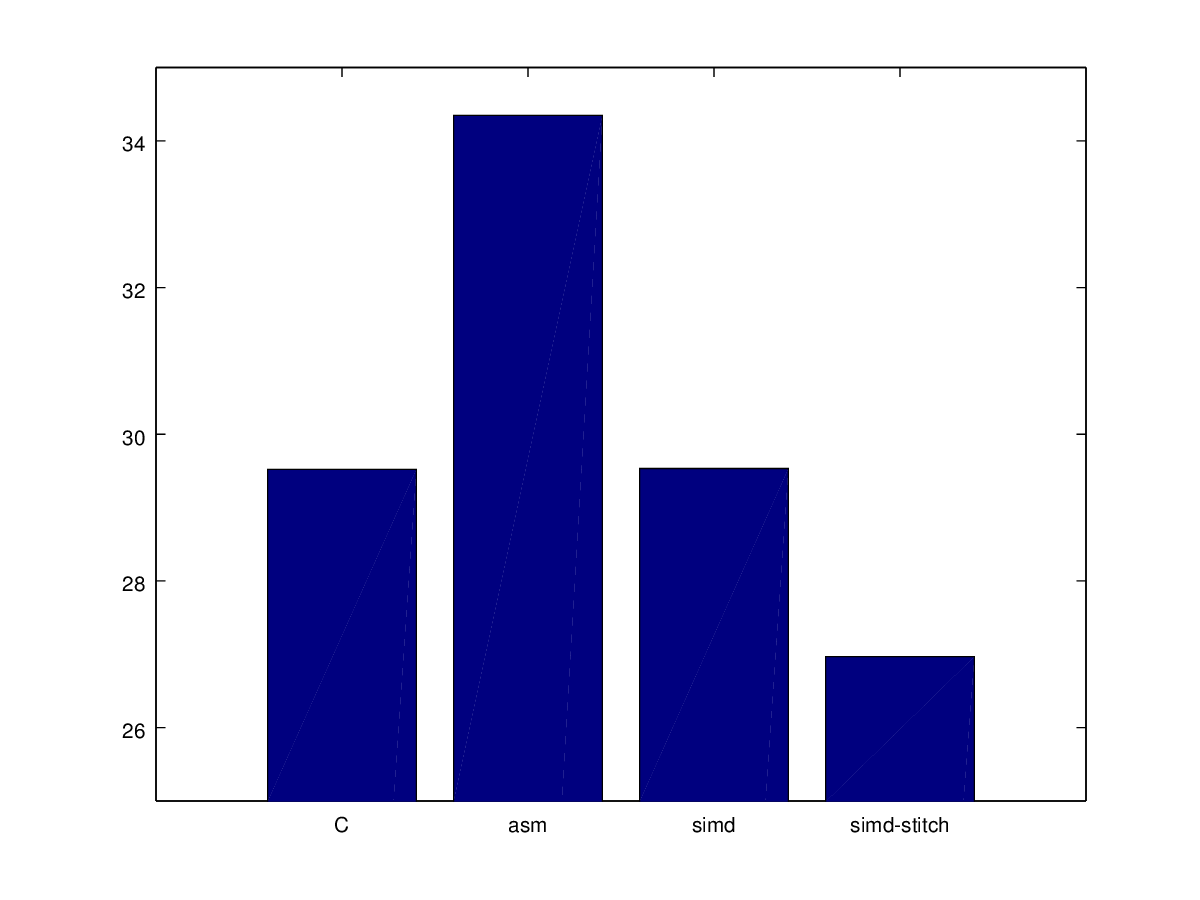
\includegraphics[scale=0.60]{sha256/imagenes/sha256-test-1.png}
    \caption{Cantidad de ciclos necesarios para aplicar el algoritmo $100000$ veces a un mensaje de un bloque ($64$ bytes) y dividiendo esa cantidad por la cantidad de bytes hasheados, es decir, $6400000$}
\end{figure}
\end{center}

\begin{center}
\begin{figure}[H]
    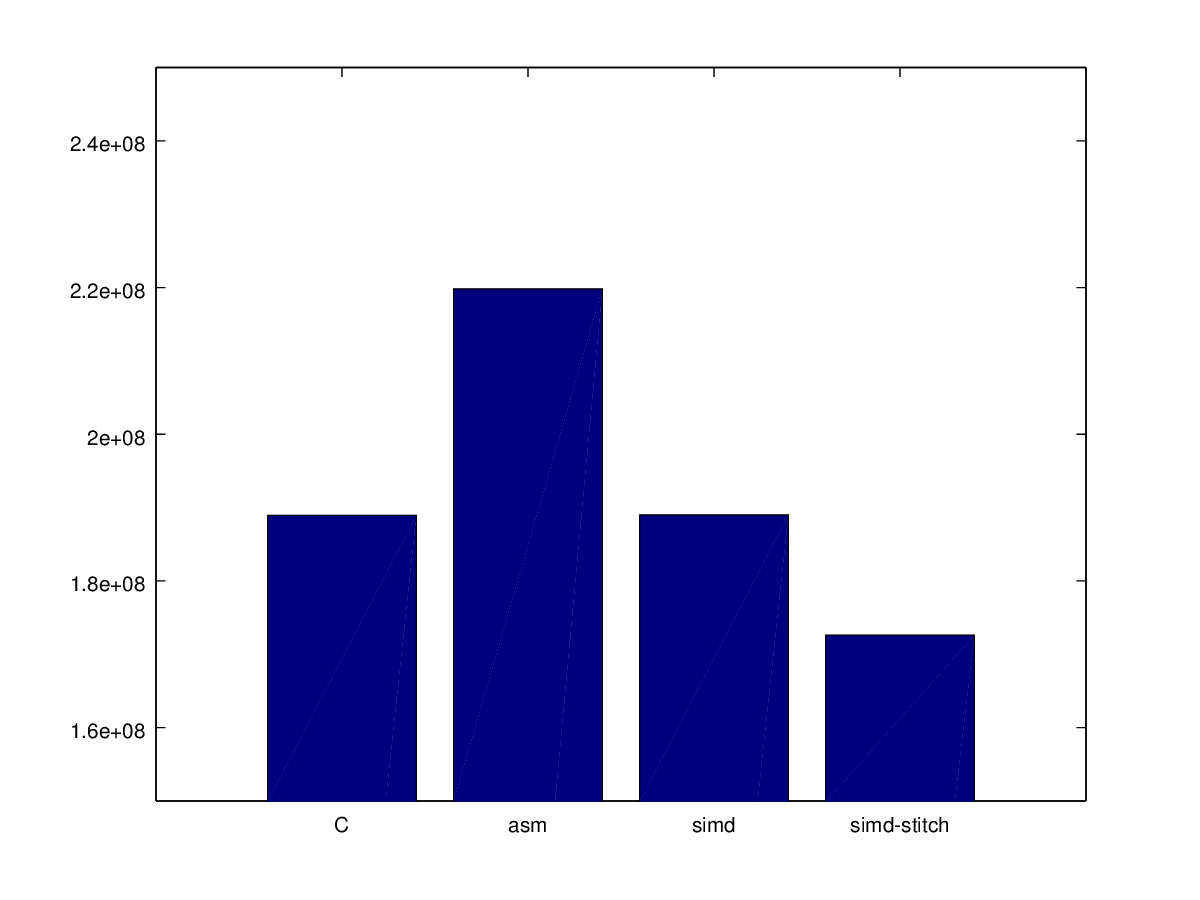
\includegraphics[scale=0.60]{sha256/imagenes/sha256-test-2.png}
    \caption{Cantidad de ciclos necesarios para aplicar el algoritmo $100000$ veces a un mensaje de un bloque ($64$ bytes)}
\end{figure}
\end{center}

Como puede verse claramente, la implementación con la mejor performance es simd-stitch, logrando reducir tiempos entre $25\%$ y $10\%$, por lo que se puede concluir que el uso de los recursos SIMD del procesador y la técnica de function stitching provocan una mejora importante en el desempeño del algoritmo. \\
\indent Como se comentó en la sección \ref{sec:impshac}, al compilar el código fuente en C usando el flag $\texttt{-O3}$, el código objeto obtenido utiliza ampliamente recursos SIMD por lo que los mejores tiempos obtenidos usando lenguaje C frente al uso de ensamblador sin SIMD podrían indicar que el buen uso de SIMD mejora el cómputo de este algoritmo. \\ \indent Teniendo en cuenta que al usar SIMD, directa o indirectamente a travéz del compilador, sin usar la técnica de function stitching, se obtienen mejoras de aproximadamente un $15\%$ (comparando la implementación simd y C con la implementación en assembler sin simd), se puede afirmar que usando de manera apropiada las instrucciones y registros de las extenciones $\texttt{sse}$, $\texttt{sse2}$, etc. de intel, se puede mejorar la performance del algoritmo sha256 de manera sustancial.\\
\indent Como conclusión general podemos decir que el uso de las capacidades SIMD de los procesadores pueden usarse para crear mejores implementaciones de la función de hash sha256.
